\documentclass[
	% -- opções da classe memoir --
	12pt,				% tamanho da fonte
	%openright,			% capítulos começam em pág ímpar (insere página vazia caso preciso)
	oneside,			% para impressão no anverso. Oposto a twoside
	a4paper,			% tamanho do papel. 
	% -- opções da classe abntex2 --
	chapter=TITLE,		% títulos de capítulos convertidos em letras maiúsculas
	section=TITLE,		% títulos de seções convertidos em letras maiúsculas
	%subsection=TITLE,	% títulos de subseções convertidos em letras maiúsculas
	%subsubsection=TITLE,% títulos de subsubseções convertidos em letras maiúsculas
	% -- opções do pacote babel --
	english,			% idioma adicional para hifenização
	%french,				% idioma adicional para hifenização
	%spanish,			% idioma adicional para hifenização
	brazil				% o último idioma é o principal do documento
	]{abntex2}

% Pacote de definições proprias
% ---
\usepackage{setup/ufscthesisA4-alf}


% Pacotes especificos
% ---
\usepackage{pgfgantt} % Gantt charts
\usepackage{calc}     % Arithmetic in LaTeX
\usepackage{tabularx} % Flexible tables
\usepackage{svg}
% Definições para usar no Gantt
\newlength{\myunitx}
\newlength{\autosizewidth}
\newcommand*{\timeslots}{}
% ---
% Pacotes de citações
% ---
\usepackage{csquotes}
\usepackage[backend = bibtex, style = abnt]{biblatex}
% FIXME Se desejar estilo numérico de citações,  comente a linha acima e descomente a linha a seguir.
% \usepackage[backend = biber, style = numeric-comp]{biblatex}

% ---
% Filtering and Mapping Bibliographies
% ---

\setlength\bibitemsep{\baselineskip}
\DeclareFieldFormat{url}{Disponível~em:\addspace\url{#1}}
\NewBibliographyString{sineloco}
\NewBibliographyString{sinenomine}
\DefineBibliographyStrings{brazil}{%
	sineloco     = {\mkbibemph{S\adddot l\adddot}},
	sinenomine   = {\mkbibemph{s\adddot n\adddot}},
	andothers    = {\mkbibemph{et\addabbrvspace al\adddot}},
	in			 = {\mkbibemph{In:}}
}

\addbibresource{aftertext/Referencias.bib} % Seus arquivos de referências

% ---
\DeclareSourcemap{
	\maps[datatype=bibtex]{
		% remove fields that are always useless
		\map{
			\step[fieldset=abstract, null]
			\step[fieldset=pagetotal, null]
		}
		% remove URLs for types that are primarily printed
%		\map{
%			\pernottype{software}
%			\pernottype{online}
%			\pernottype{report}
%			\pernottype{techreport}
%			\pernottype{standard}
%			\pernottype{manual}
%			\pernottype{misc}
%			\step[fieldset=url, null]
%			\step[fieldset=urldate, null]
%		}
		\map{
			\pertype{inproceedings}
			% remove mostly redundant conference information
			\step[fieldset=venue, null]
			\step[fieldset=eventdate, null]
			\step[fieldset=eventtitle, null]
			% do not show ISBN for proceedings
			\step[fieldset=isbn, null]
			% Citavi bug
			\step[fieldset=volume, null]
		}
	}
}
% ---

% ---
% Informações de dados para CAPA e FOLHA DE ROSTO
% ---
\titulo{RAPID - Rocket with Affordable Propellant Injection Design}
\subtitulo{Design Preliminar de Motor-Foguete Bi-Propelente Liquido com Bombeamento Elétrico}
\autor{Antônio Otaviano Dourado}
\local{Joinville}
\data{31 de Julho de 2025}
\ano{2025}
\instituicaosigla{UFSC}
\instituicao{Universidade Federal de Santa Catarina}
\tipotrabalho{Proposta de projeto de pesquisa}
\programa{Departamento de Engenharias da Mobilidade}
\centro{Centro Tecnológico de Joinville}
\preambulo
{%
\imprimirtipotrabalho~submetido ao~\imprimirprograma~da~\imprimirinstituicao.
}
% ---

% ---
% Configurações de aparência do PDF final
% ---
% alterando o aspecto da cor azul, de acordo com identidade visual da UFSC
\definecolor{blue}{RGB}{0,56,147}

% informações do PDF
\makeatletter
\hypersetup{
     	%pagebackref=true,
		pdftitle={\@title}, 
		pdfauthor={\@author},
    	pdfsubject={\imprimirpreambulo},
	    pdfcreator={Grupo RAPID},
		pdfkeywords={projeto de pesquisa}{RAPID}{UFSC}, 
		colorlinks=true,       		% false: boxed links; true: colored links
    	linkcolor=blue,          	% color of internal links
    	citecolor=blue,        		% color of links to bibliography
    	filecolor=magenta,      		% color of file links
		urlcolor=blue,
		bookmarksdepth=4
}
\makeatother
% --- 


% ---
% compila a lista de abreviaturas e siglas e a lista de símbolos
% ---

% Declaração das siglas
\siglalista{RAPID}{\textit{Rocket with Affordable Propellant Injection Design}}
\siglalista{EPFS}{\textit{Electric Pump Feed System}}
\siglalista{EthaLOx}{Etanol - Oxigênio Líquido}
\siglalista{RoCAT}{\textit{Rocket Cycle Analysis Tool}}
\siglalista{AM}{\textit{Additive Manufacturing}}
\siglalista{UFSC}{Universidade Federal de Santa Catarina}
\siglalista{IAE}{Instituto de Aeronáutica e Espaço}
\siglalista{MBSE}{\textit{Model Based Systems Engineering}}

% Declaração dos simbolos
\simbololista{C}{\ensuremath{C}}{Circunferência de um círculo}
\simbololista{pi}{\ensuremath{\pi}}{Número pi} 
\simbololista{r}{\ensuremath{r}}{Raio de um círculo}
\simbololista{A}{\ensuremath{A}}{Área de um círculo}

% compila a lista de abreviaturas e siglas e a lista de símbolos
\makenoidxglossaries 

% ---

% ---
% compila o indice
% ---
\makeindex
% ---

% ----
% Início do documento
% ----
\begin{document}

% Seleciona o idioma do documento (conforme pacotes do babel)
%\selectlanguage{english}
\selectlanguage{brazil}

% Retira espaço extra obsoleto entre as frases.
\frenchspacing 

% Espaçamento 1.5 entre linhas
\OnehalfSpacing

% Corrige justificação
%\sloppy

% ----------------------------------------------------------
% ELEMENTOS PRÉ-TEXTUAIS
% ----------------------------------------------------------
% \pretextual %a macro \pretextual é acionado automaticamente no início de \begin{document}
% ---
% Capa, folha de rosto, ficha bibliografica, errata, folha de apróvação
% Dedicatória, agradecimentos, epígrafe, resumos, listas
% ---
% ---
% Capa
% ---
\imprimircapa
% ---

% ---
% Folha de rosto
% (o * indica que haverá a ficha bibliográfica)
% ---
\imprimirfolhaderosto*
% ---


{%hidelinks
	\hypersetup{hidelinks}
	% ---
	% inserir lista de ilustrações
	% ---
	%\pdfbookmark[0]{\listfigurename}{lof}
	%\listoffigures*
	%\cleardoublepage
	% ---
	
	% ---
	% inserir lista de quadros
	% ---
	%\pdfbookmark[0]{\listofquadrosname}{loq}
	%\listofquadros*
	%\cleardoublepage
	% ---
	
	% ---
	% inserir lista de tabelas
	% ---
	%\pdfbookmark[0]{\listtablename}{lot}
	%\listoftables*
	%\cleardoublepage
	% ---
	
	% ---
	% inserir lista de abreviaturas e siglas (devem ser declarados no preambulo)
	% ---
	\imprimirlistadesiglas
	% ---
	
	% ---
	% inserir lista de símbolos (devem ser declarados no preambulo)
	% ---
	%\imprimirlistadesimbolos
	% ---
	
	% ---
	% inserir o sumario
	% ---
	\pdfbookmark[0]{\contentsname}{toc}
	\tableofcontents*
	\cleardoublepage
	
}%hidelinks
% ---
% ---

% ----------------------------------------------------------
% ELEMENTOS TEXTUAIS
% ----------------------------------------------------------
\textual
% ---
\chapter{Introdução}

O desenvolvimento de motores-foguete a propelente líquido é um dos principais desafios técnico-científicos enfrentados por países que buscam a autonomia em sistemas de lançamento espacial. Apesar do Brasil possuir um histórico consolidado no desenvolvimento de motores a propelente sólido, avançar na tecnologia de propulsão líquida é essencial para a competitividade no cenário espacial internacional, principalmente em aplicações que demandam maior eficiência, controle e flexibilidade de operação.

Entre os diversos ciclos termodinâmicos possíveis em motores-foguete de propelente líquido, destaca-se o ciclo com bombeamento elétrico dos propelentes, \Gls{EPFS}, recentemente viabilizado devido ao avanço significativo da densidade de energia de baterias comerciais, impulsionado pela indústria automobilística. Diferente de sistemas clássicos com turbobombas acionadas por turbinas a gás, o ciclo \Gls{EPFS} emprega motores elétricos alimentados por baterias para acionar as bombas de combustível e oxidante. Essa abordagem apresenta uma série de vantagens: redução da complexidade mecânica e dos custos de desenvolvimento, facilidade de controle e de partida, e potencial de modularização do sistema \cite{liuConceptKeyTechnology2021a}.

Entretanto, essas vantagens vêm acompanhadas de desafios significativos relacionados à densidade de massa e à eficiência do sistema de armazenamento de energia elétrica, o que impõe limites à aplicação do ciclo em missões de longa duração ou alto desempenho. Estudos recentes demonstram que, embora o ciclo \Gls{EPFS} apresente maior massa veicular para determinadas condições, ele pode oferecer melhor relação desempenho/custo para faixas intermediárias de empuxo e tempo de queima, especialmente em estágios superiores ou sistemas reutilizáveis \cite{Berg2023}.

A proposta do projeto \Gls{RAPID} visa investigar e desenvolver o projeto preliminar de um motor-foguete bi-propelente com bombeamento elétrico, voltado à aplicação didático-experimental e ao suporte de futuras fases de pesquisa em propulsão líquida. O projeto pretende construir uma base tecnológica nacional no desenvolvimento de sistemas de injeção e alimentação de propelente, com foco na simplicidade de fabricação, robustez e potencial de evolução para aplicações mais complexas. A escolha pelo ciclo com bombeamento elétrico se justifica pela alta viabilidade de desenvolvimento em ambiente universitário, além da crescente relevância desse ciclo no cenário internacional, como demonstrado pelo sucesso comercial do foguete Electron da empresa Rocket Lab \cite{RocketLab2017}.

\section{Problema e Justificativa}

O Brasil carece de iniciativas consistentes voltadas à formação de especialistas e à estruturação de infraestrutura laboratorial voltada ao desenvolvimento de motores a propelente líquido. Apesar de projetos como o L75, conduzido pelo \Gls{IAE}, terem alcançado marcos importantes, ainda há espaço para o fortalecimento de iniciativas acadêmicas com foco em projetos de menor escala, que permitam ciclos mais curtos de experimentação e aprendizado \cite{DevL75}.

Neste contexto, a escolha pelo ciclo \Gls{EPFS} se apresenta como alternativa estratégica. A eliminação do uso de turbinas e geradores de gás permite a redução dos riscos e da complexidade associada ao desenvolvimento de um motor funcional, além de facilitar a implementação de sistemas de controle baseados em eletrônica embarcada. Além disso, a arquitetura \Gls{EPFS} permite estudar tecnologias de bombas, injetores e câmaras de combustão de forma modular.

A escolha do par propelente \Gls{EthaLOx} se justifica por sua combinação favorável de alto desempenho específico, baixo custo e acessibilidade no contexto nacional. Além de não serem tóxicos, esses propelentes possuem propriedades que facilitam sua utilização em aplicações educacionais e em testes repetitivos \cite{DevL75}.

\section{Objetivos}

\subsection{Objetivo Geral}

Desenvolver o projeto preliminar de um motor-foguete a propelente líquido com bombeamento elétrico, de pequeno porte, voltado à experimentação de tecnologias de injeção, combustão e pressurização de propelentes.

\subsection{Objetivos Específicos}

\begin{itemize}

\item Definir os requisitos preliminares do sistema de propulsão;

\item Modelar e otimizar os subsistemas principais do motor (bombas, injetores, câmara de combustão); \item Elaborar o projeto preliminar dos subsistemas;

\item Avaliar o desempenho do ciclo \Gls{EPFS} e suas limitações práticas;

\end{itemize}

Este projeto representa um passo inicial em uma linha de pesquisa com potencial de expansão, abrindo caminho para colaborações interinstitucionais e futuras propostas de financiamento para a construção e teste dos sistemas projetados.
% ---
\chapter{Metas e Resultados}

\section{Metas}

\begin{itemize}
    \item Estabelecer os requisitos preliminares do motor-foguete com ciclo \gls{EPFS} e par propelente \Gls{EthaLOx};
    \item Desenvolver modelos computacionais dos principais subsistemas (bombas, injetores, câmara de combustão) e realizar sua otimização;
    \item Elaborar o design preliminar dos subsistemas do motor com foco em viabilidade de fabricação e segurança operacional;
    \item Publicar ao menos 2 artigos científicos relacionados a subsistemas e modelagem de motores-foguete de propelente líquido;
    \item Publicar ao menos 2 artigos científicos especificamente sobre arquitetura e desempenho de sistemas com bombeamento elétrico;
    \item Participar de eventos científicos e técnicos nacionais e internacionais;
    \item Ampliar a visibilidade institucional da UFSC na área de propulsão líquida.
\end{itemize}

\section{Resultados Esperados}

\begin{itemize}
    \item Documento técnico com os requisitos preliminares do motor-foguete RAPID;
    \item Publicação de artigo: \textit{"Requisitos Preliminares de Motor-Foguete Bi-Propelente com Bombeamento Elétrico"};
    \item Modelos validados e resultados de simulações dos subsistemas principais;
    \item Publicação de artigo: \textit{"Design Preliminar de Motor-Foguete Bi-Propelente com Bombeamento Elétrico"};
    \item Apresentações em congressos e simpósios de engenharia aeroespacial;
\end{itemize}
% ---
\chapter{Metodologia}
\section{Caracterização do Objeto de Estudo}\label{sec:carac}
O objeto de estudo deste projeto é o design preliminar do motor-foguete de propelente líquido alimentado com \gls{EthaLOx}, desenvolvido para fins acadêmicos e experimentais. Trata-se de um sistema de propulsão de pequeno porte, com empuxo médio estimado de 1 kN, concebido como base para pesquisa e desenvolvimento de tecnologias aplicadas a motores-foguete. O projeto está sendo conduzido por estudantes da \Gls{UFSC} com o objetivo de consolidar conhecimento técnico nas áreas de injeção, resfriamento, alimentação de propelentes, controle e desempenho térmico-estrutural.

O motor será operado em ciclo \gls{EPFS}, buscando simplicidade de implementação e controle, além de maior compatibilidade com estudos acadêmicos de laboratório. A escolha dos propelentes baseia-se em critérios de disponibilidade, propriedades termoquímicas e maturidade tecnológica, sendo o etanol adotado como combustível e o oxigênio líquido como oxidante.

O objeto de estudo é abordado exclusivamente em nível teórico e analítico, com foco na definição de parâmetros de projeto, critérios de dimensionamento e integração dos subsistemas. As soluções técnicas estudadas consideram a aplicação de manufatura aditiva, ou \gls{AM}, metálica, superfícies de transferência de calor otimizadas, injetores com geometrias compatíveis com \gls{AM} e válvulas criogênicas compactas. A ênfase está na avaliação do comportamento funcional de cada subsistema dentro de um cenário teórico de operação, sem execução de testes físicos nem produção de protótipos nesta etapa.

O estudo do motor-foguete como objeto central permite a investigação coordenada de múltiplos aspectos da engenharia aeroespacial, incluindo transferência de calor em canais regenerativos, desempenho de bombas e impulsores, estabilidade de combustão, escolha de materiais e integração térmica de componentes submetidos a altos gradientes de temperatura e pressão.

\section{Universo de Pesquisa}\label{sec:univ}
A pesquisa concentra-se no desenvolvimento de soluções técnicas aplicáveis a motores de pequeno porte voltados à propulsão experimental, sem aplicação direta em sistemas comerciais ou operacionais previstas inicialmente, mas com conceitos e tecnologia que podem ser escalados a demais projetos. As atividades serão conduzidas por meio de levantamento bibliográfico, modelagem teórica e análise de viabilidade de subsistemas, sem realização de testes físicos ou experimentação prática, mas sim por meio de estudos conceituais e simulações de fenômenos e design a serem analisados.

\section{Estudos Propostos}\label{sec:estudos}
O projeto \Gls{RAPID} encontra-se em fase inicial, com foco na definição de pré-requisitos técnicos e no desenvolvimento conceitual dos principais subsistemas de um motor-foguete de propelente líquido, com empuxo médio estimado de 1 kN, utilizando etanol e oxigênio líquido como propelentes. Esta etapa visa estabelecer a base teórica e os parâmetros de projeto necessários para o avanço das atividades de desenvolvimento.

\section{Abordagem de Gerenciamento de Equipe}\label{sec:geren}
A gestão do trabalho entre os membros do projeto \Gls{RAPID} será conduzida com base na metodologia ágil, utilizando o \textit{framework} Scrum como modelo organizacional. A estrutura de Scrum adotada prevê ciclos quinzenais, com duração de quinze dias, coincidentes com as etapas previstas no Cronograma Físico (Anexo~\ref{cronograma}) do projeto e na subdivisão apresentada na seção \ref{sec:fases}. Essa sincronização permite que a organização do trabalho individual e coletivo esteja diretamente vinculada às entregas esperadas em cada fase do projeto.

O Scrum é um modelo de gestão ágil iterativo e incremental, originalmente desenvolvido para projetos de software, mas amplamente adotado em ambientes de engenharia e pesquisa. Ele estabelece papéis claros, rituais periódicos e priorização contínua de tarefas~\cite{Bott2020}. No contexto do projeto \Gls{RAPID}, cada ciclo, de duração quinzenal, inclui a definição de tarefas a serem desenvolvidas, a revisão de entregas anteriores e a reavaliação de prioridades com base nas dependências técnicas e nas metas de desenvolvimento. O foco está na flexibilidade, no acompanhamento contínuo e na divisão eficiente do trabalho entre os membros da equipe.

A organização das tarefas será feita por meio de um sistema visual de kanban, utilizando a plataforma gratuita \textit{Deck}, que centraliza a gestão de tarefas individuais e coletivas. O \textit{Deck} está integrado a um servidor privado que reúne a infraestrutura digital da equipe, incluindo documentação técnica, bibliografia de referência, controle de versões, organização de arquivos, registros de reuniões e acompanhamento do progresso. Esse sistema garante rastreabilidade, consistência e facilidade de acesso às informações por todos os integrantes, mesmo em atividades assíncronas.

A abordagem de gerenciamento de equipe está estruturada para garantir autonomia operacional, priorização clara de atividades e capacidade de adaptação contínua, respeitando as características de um ambiente de pesquisa e projeto. A organização individual do trabalho está vinculada à execução das tarefas técnicas previstas na secção \ref{sec:metod}, que detalha a lógica de desenvolvimento adotada no \Gls{RAPID}.

\section{Abordagem Metodológica do Projeto}\label{sec:metod}

A condução metodológica do projeto \Gls{RAPID} é baseada no modelo de gerenciamento de tecnologia da NASA, o NPR 7120.8A \cite{NASAResearchTechnology2018}, adaptado para o contexto acadêmico de desenvolvimento de um sistema de propulsão líquido de pequeno porte. O ciclo de desenvolvimento adotado segue uma abordagem iterativa e evolutiva, típica de processos de engenharia de design, priorizando flexibilidade, refinamento progressivo e validação conceitual.

\begin{figure}[h!]
    \centering
    \caption{Mapa do processo de pesquisa de design preliminar adotado no projeto \Gls{RAPID}.}
    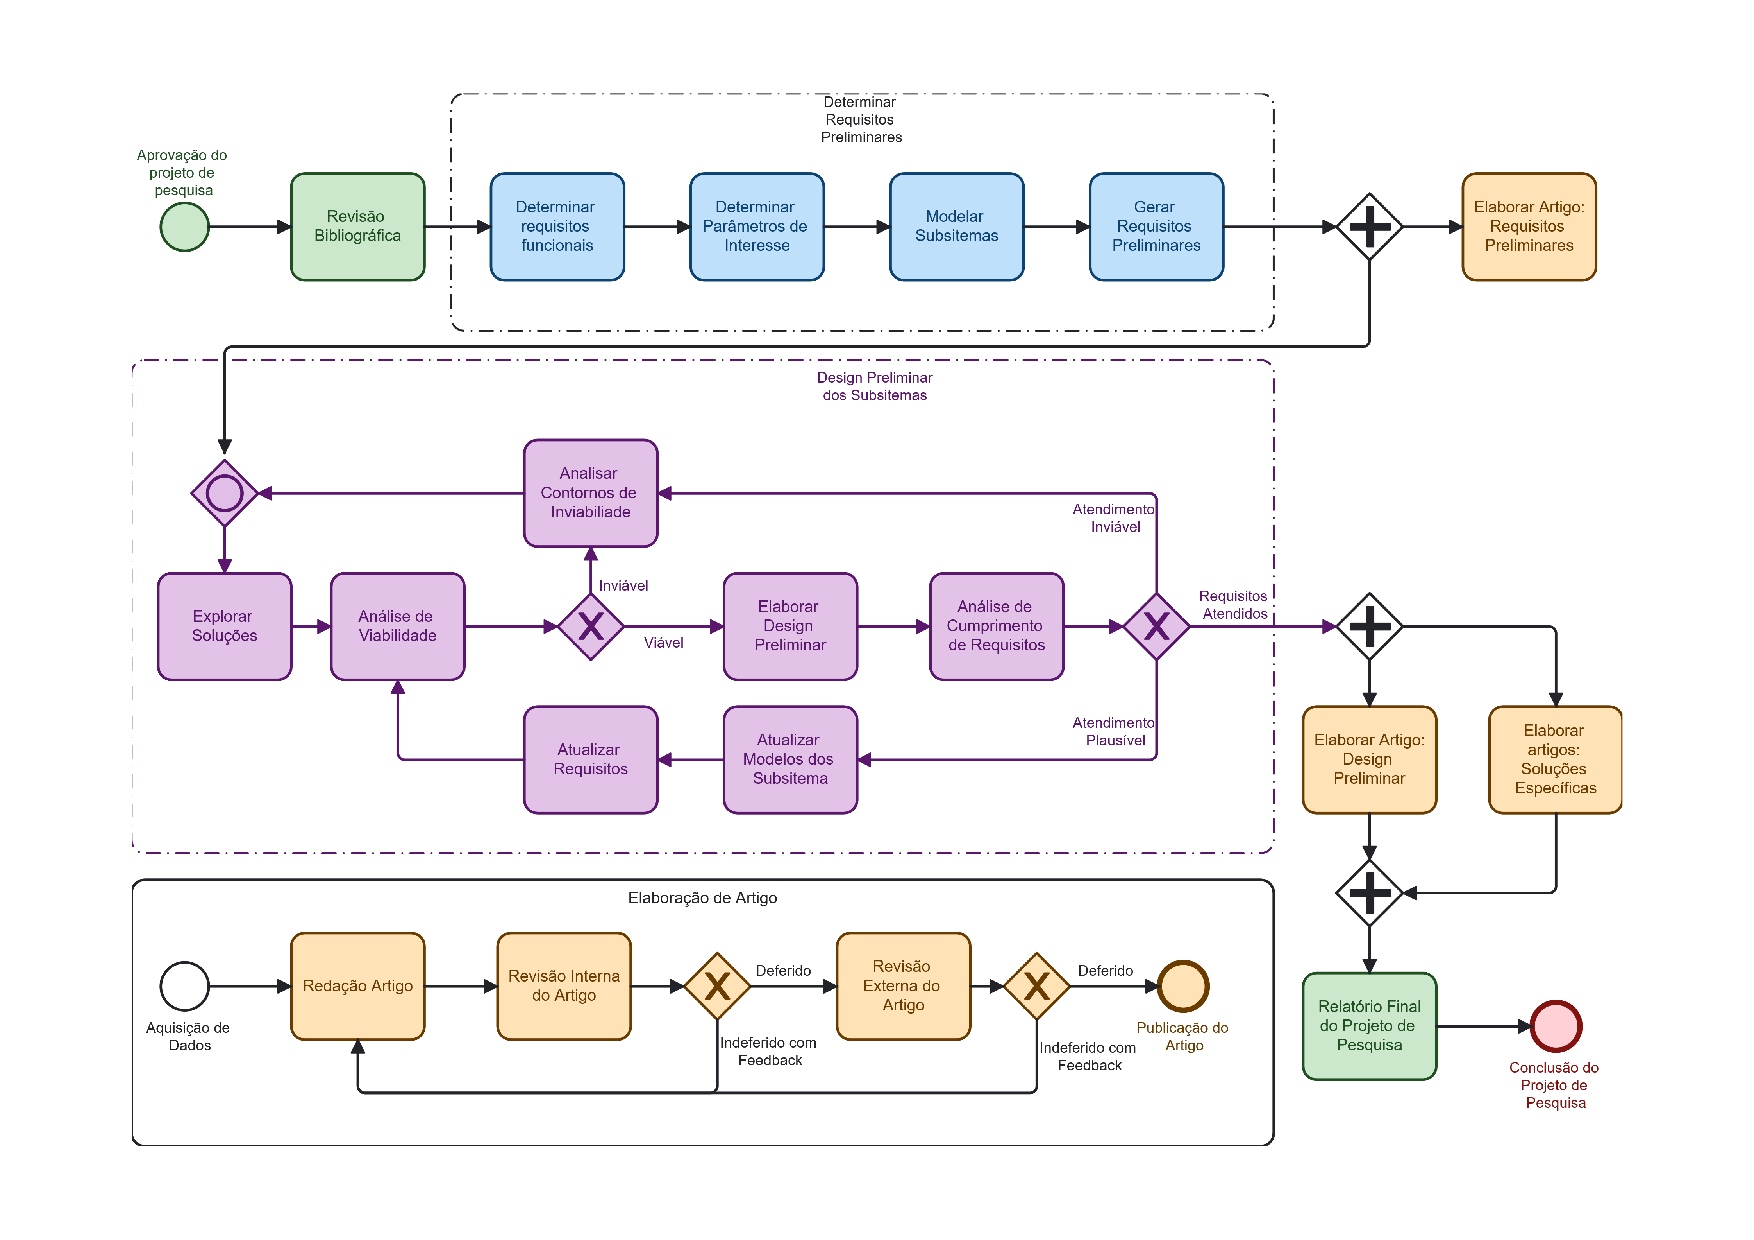
\includegraphics[width=0.85\textwidth]{Imagens/ProcessoDePesquisaDeDesign}
    \fonte{Elaborado pelo Autor (2025).}
    \label{fig:bpmn}
\end{figure}

O processo metodológico é representado na Figura~\ref{fig:bpmn}, que ilustra o ciclo de pesquisa em design adotado no projeto. Esse ciclo compreende iterações sucessivas entre as atividades de modelagem, análise, proposição de soluções e revisão. Isso permite uma adaptação contínua das soluções técnicas em função dos requisitos, restrições e novas descobertas.

Além disso, o projeto adota uma abordagem de desenvolvimento baseada em modelos, conhecida como \Gls{MBSE}. Essa abordagem permite que modelos matemáticos e computacionais sirvam como elementos centrais na definição, análise e validação do sistema como um todo. O uso do \Gls{MBSE} contribui para maior rastreabilidade, consistência entre requisitos e soluções e suporte à tomada de decisão durante as fases de projeto \cite{EstefanMBSE2008}.

\begin{figure}[h!]
    \centering
    \caption{Exemplo de diagrama esquemático de performance de um motor \gls{EPFS} otimizado com \gls{RoCAT}.}
    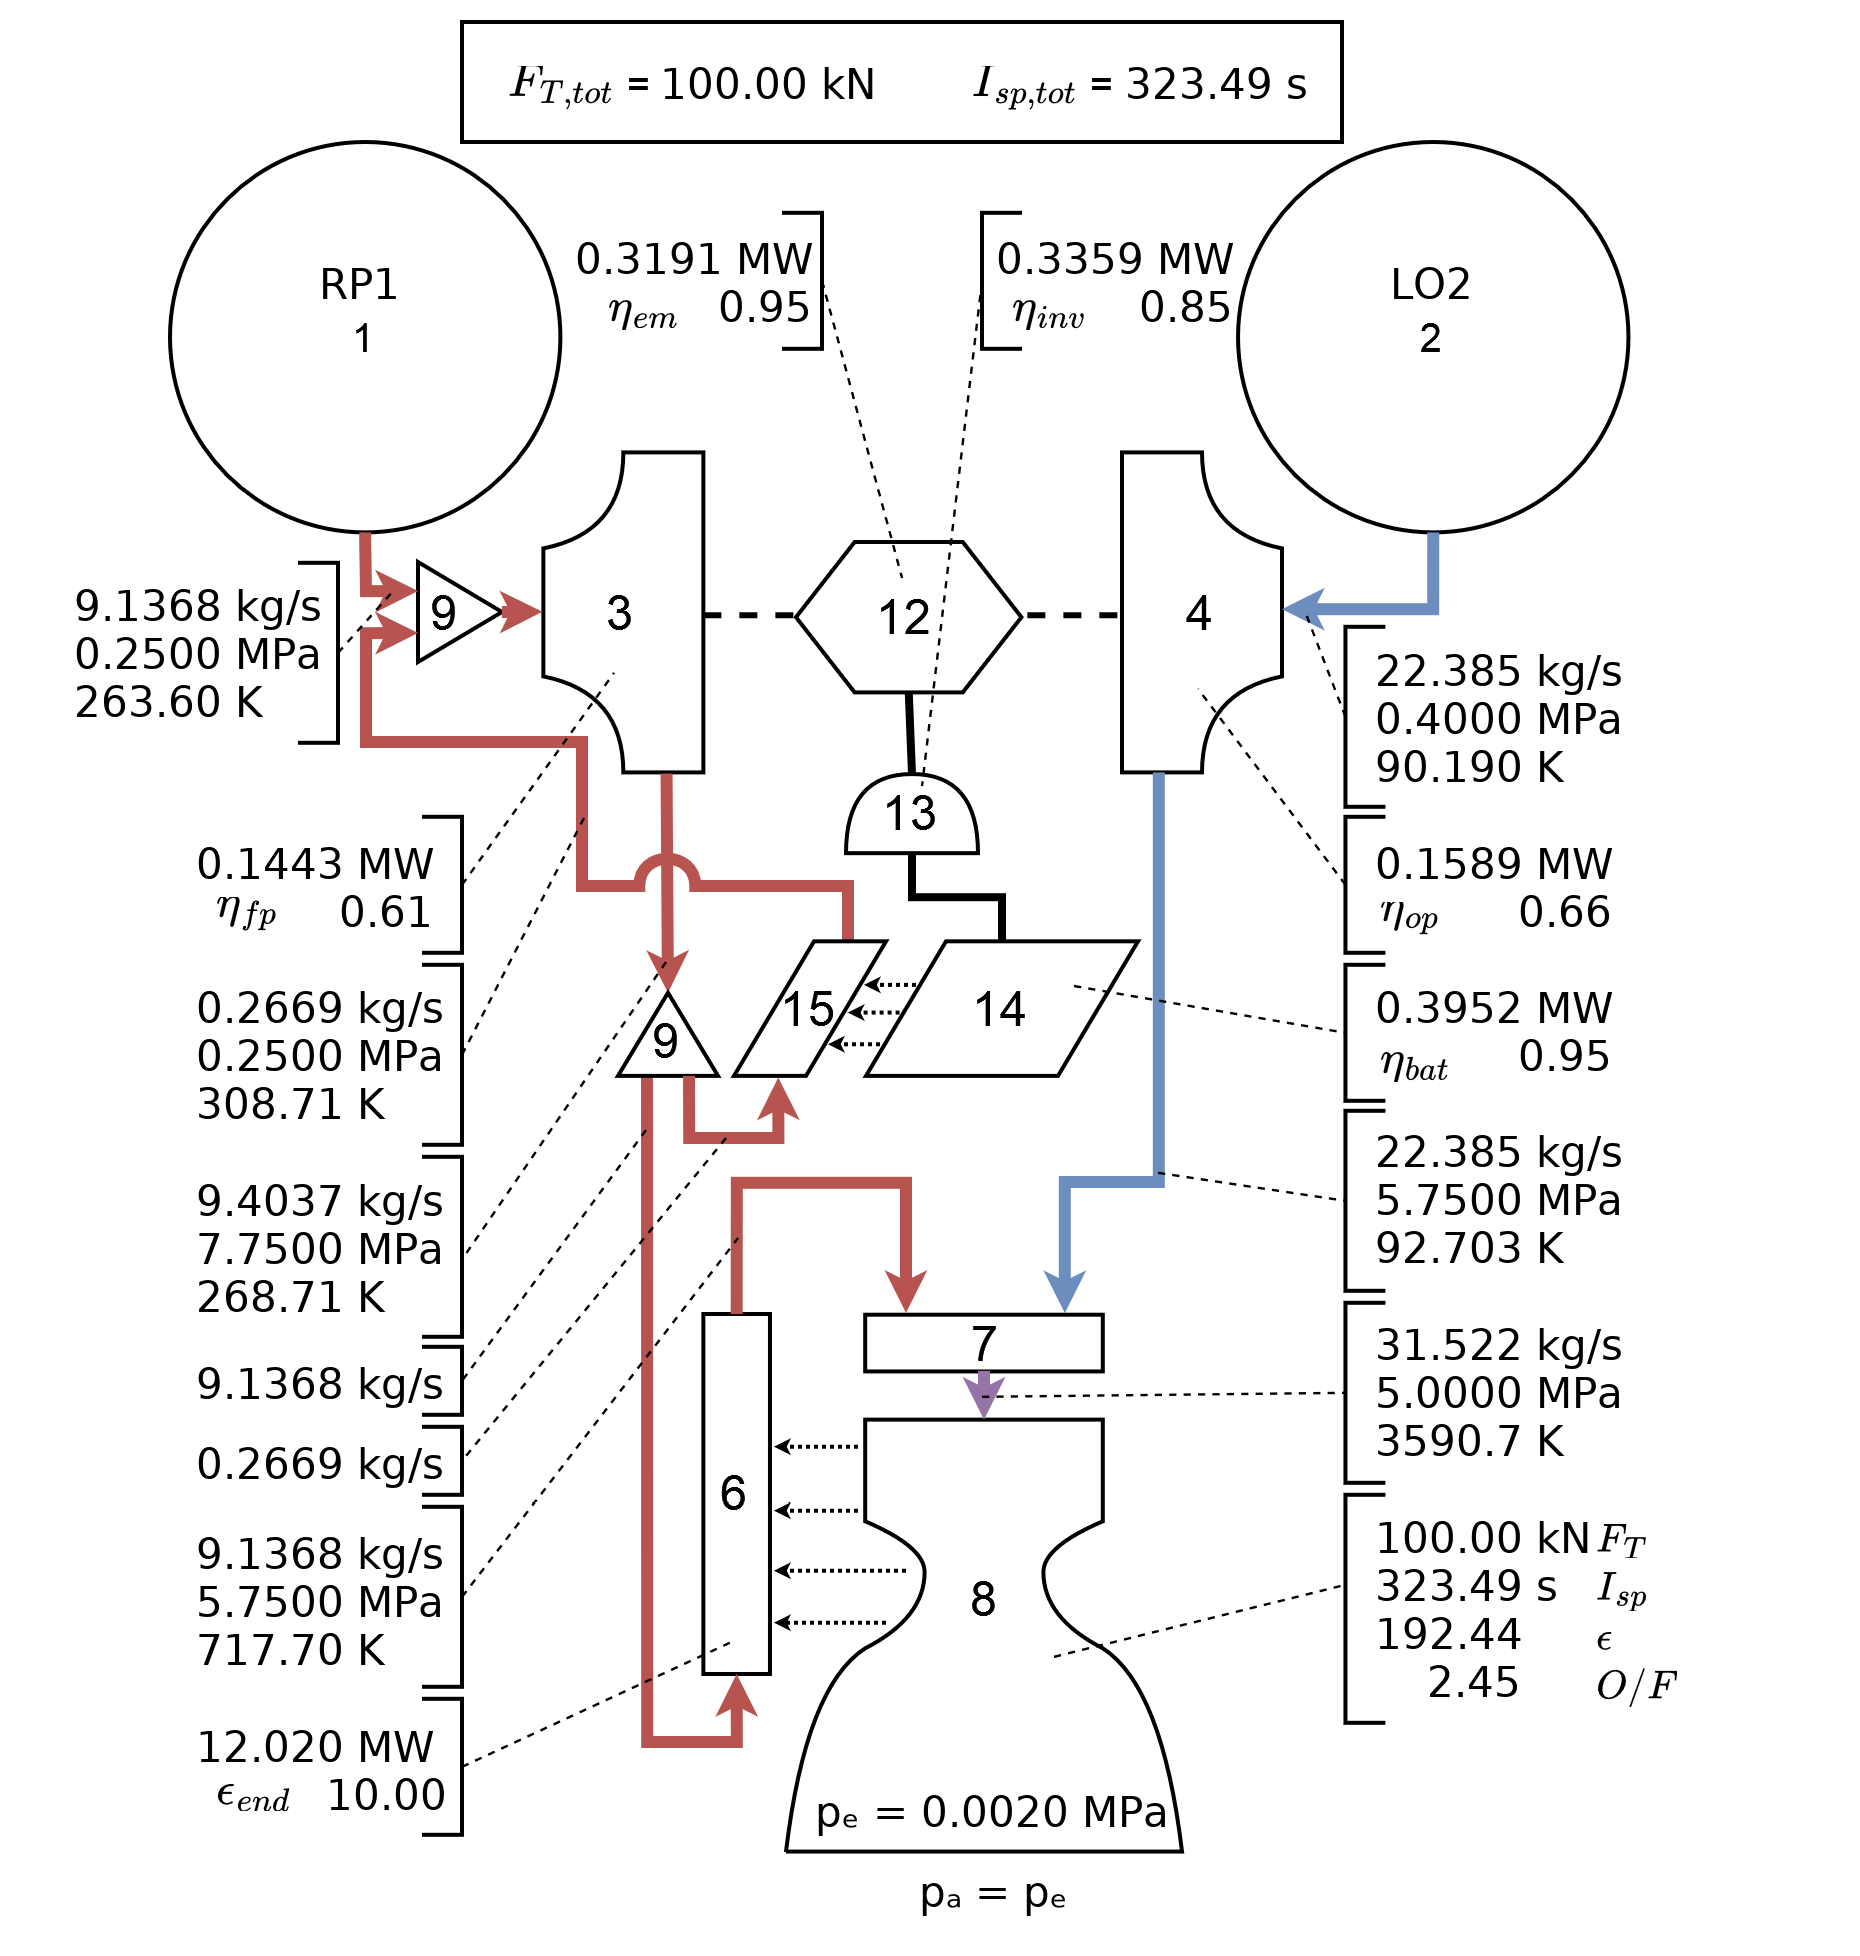
\includegraphics[width=0.85\textwidth]{Imagens/EPFS.png}
    \fonte{\textcite{Berg2023}}
    \label{fig:EPFS}
\end{figure}

No caso específico do \Gls{RAPID}, será desenvolvido um modelo matemático do sistema de propulsão, com foco no ciclo \gls{EPFS} e em sua interação com os subsistemas de alimentação, combustão e resfriamento. Um exemplo de representação funcional desse modelo pode ser visto na Figura~\ref{fig:EPFS}, onde se observa a lógica de operação e os parâmetros envolvidos na otimização de performance com a ferramenta \gls{RoCAT}.

As fases de projeto estão organizadas de modo a permitir adaptação dinâmica dos objetivos técnicos conforme os resultados obtidos em cada iteração. Essa estrutura favorece a aprendizagem contínua, a integração progressiva dos subsistemas e o amadurecimento gradual da solução até o design preliminar consolidado.

\section{Decomposição do Trabalho}\label{sec:trabalho}
O plano de trabalho, representado no cronograma apresentado no Anexo~\ref{cronograma}, está estruturado em três fases lógicas e interdependentes, permitindo a condução sequencial e controlada das atividades. Essa segmentação viabiliza a definição de marcos intermediários e a entrega de resultados concretos em cada etapa, alinhando-se a boas práticas de gerenciamento de projetos.

Cada fase foi subdividida em sub-fases específicas, cuja conclusão está associada a marcos técnicos internos que têm por objetivo revisar o progresso, validar os requisitos definidos e orientar ajustes no escopo técnico conforme necessário.

No contexto da abordagem metodológica do projeto, os marcos técnicos estarão associados a análises formais de progresso, validação de soluções desenvolvidas e consolidação de decisões técnicas. Esses marcos têm como objetivo orientar o refinamento do projeto, registrar o estado de maturidade técnica e fundamentar a produção de documentos ou estudos que sustentem as próximas etapas do desenvolvimento.


\section{Estrutura de Fases}\label{sec:fases}

Antes do início das fases, foi definido um período equivalente a dois ciclos de Scrum, reservado exclusivamente para a revisão bibliográfica dos temas listados para pesquisa. A partir dessa revisão e da sistematização das informações pelos membros da equipe, foram estabelecidos os fundamentos técnicos que orientam a organização do projeto. Com base nisso, as fases foram iniciadas e seguem a seguinte estrutura:

\subsection{Fase I: Revisão Bibliográfica}
Essa etapa tem como foco a fundamentação técnica e a definição dos temas específicos de estudo. Duração estimada de dois Ciclos Scrum.

\subsection{Fase II: Estabelecimento de Parâmetros e Requisitos de Projeto}

Esta fase tem como objetivo estabelecer os parâmetros iniciais e as condições de contorno que orientarão o desenvolvimento dos subsistemas do motor. A definição será guiada pela análise dos objetivos do projeto, pela caracterização funcional esperada e pelas condições de operação previstas, levando em conta restrições ambientais, materiais e construtivas.

\subsubsection{Sub-fase II.1: Identificação e Classificação de Parâmetros de Interesse}
Nesta sub-fase, a equipe deverá listar os parâmetros termodinâmicos e operacionais relevantes ao desempenho do sistema, como pressão de câmara, taxa de mistura e temperatura de operação. Esses parâmetros serão classificados como variáveis livres (passíveis de otimização) ou fixos, quando determinados por restrições externas ou limitações técnicas. Não será feita a definição de seus valores numéricos nesta etapa, apenas sua seleção e categorização para orientar a modelagem e análise futuras.

\subsubsection{Sub-fase II.2: Formulação de Requisitos Funcionais dos Subsistemas}
Com base na classificação dos parâmetros e nas condições de operação previstas, a equipe deverá estabelecer os requisitos funcionais de cada subsistema. Esses requisitos definirão as condições que os componentes deverão atender para garantir segurança, desempenho e integridade estrutural — por exemplo, compatibilidade de materiais com oxigênio líquido, faixas admissíveis de temperatura e pressão, e tolerâncias dimensionais. A formulação será baseada em normas técnicas, catálogos industriais e referências científicas.

\subsubsection{Sub-fase II.3: Modelagem Teórica dos Subsistemas}
A equipe deverá realizar a modelagem analítica e o dimensionamento preliminar dos principais subsistemas com base nos requisitos funcionais definidos, considerando propriedades termodinâmicas, mecânicas e estruturais dos materiais selecionados.

\subsubsection{Sub-fase II.4: Otimização Paramétrica do Sistema}
Nesta etapa, serão utilizados os modelos desenvolvidos nas sub-fases anteriores em conjunto com ferramentas computacionais, como o \gls{RoCAT}, para explorar o espaço de soluções viáveis. O objetivo é refinar os parâmetros livres definidos na Sub-fase II.1 de modo a maximizar o desempenho global do sistema, respeitando os requisitos funcionais estabelecidos. A abordagem adotada visa facilitar iterações subsequentes no ciclo de desenvolvimento.

\subsubsection{Sub-fase II.5: Publicação dos Requisitos Preliminares}
Os resultados da Fase II serão consolidados em um artigo técnico, contendo a justificativa dos requisitos definidos, os modelos utilizados e os parâmetros estimados. Esta publicação marcará o encerramento da etapa de definição de requisitos e servirá de base para as fases subsequentes do projeto.

\subsection{Fase III: Design Preliminar dos Subsistemas}

O design dos subsistemas será conduzido por meio de um \textbf{ciclo iterativo de desenvolvimento}, com refinamento sucessivo das soluções técnicas. Não será adotado um número fixo de iterações; ao contrário, o ciclo se repetirá conforme necessidade até que as soluções atendam aos requisitos definidos. Cada iteração inclui a proposição de soluções, simulação, análise de desempenho e revisão.

\begin{itemize}
\item Proposta inicial de arquitetura de subsistemas;
\item Modelagem geométrica e funcional;
\item Verificação contra requisitos;
\item Ajuste e reiteração do design.
\end{itemize}

Essa abordagem reflete o ciclo ilustrado na Figura~\ref{fig:bpmn}, permitindo refinamento progressivo e exploração de soluções alternativas.

\subsection{Fase IV: Elaboração e Publicação de Artigos}

Etapa final com foco na documentação e divulgação dos resultados do design preliminar assim como de soluções específicas encontradas, incluindo estruturação de artigos científicos e submissões a periódicos ou eventos especializados.
% ---
\chapter{Recursos Necessários}

O projeto de pesquisa de \imprimirsubtitulo{} conta exclusivamente com a participação de voluntários, estudantes de graduação vinculados à \gls{UFSC}, sem vínculo empregatício ou remuneração financeira direta. A natureza colaborativa do projeto está alinhada aos objetivos acadêmicos e formativos, permitindo que os participantes desenvolvam competências técnicas e científicas em um ambiente multidisciplinar de pesquisa aplicada.


% ----------------------------------------------------------
% ELEMENTOS PÓS-TEXTUAIS
% ----------------------------------------------------------
\postextual
% ----------------------------------------------------------

% ----------------------------------------------------------
% Referências bibliográficas
% ----------------------------------------------------------
\begingroup
    \SingleSpacing\printbibliography[title=REFERÊNCIAS]
\endgroup

% ----------------------------------------------------------
% Glossário
% ----------------------------------------------------------
%
% Consulte o manual da classe abntex2 para orientações sobre o glossário.
%
%\glossary

% ----------------------------------------------------------
% Apêndices
% ----------------------------------------------------------

% ---
% Inicia os apêndices
% ---
%\begin{apendicesenv}
%	\partapendices* 
%	\input{aftertext/apendice_a}
%\end{apendicesenv}
% ---


% ----------------------------------------------------------
% Anexos
% ----------------------------------------------------------

% ---
% Inicia os anexos
% ---
\begin{anexosenv}
	\partanexos*
	\chapter{Cronograma físico}
\label{cronograma}
\centering
\definecolor{barblue}{RGB}{153,204,254}
\definecolor{groupblue}{RGB}{0,56,147}
\definecolor{linkred}{RGB}{165,0,33}
\renewcommand\sfdefault{phv}
\renewcommand\mddefault{mc}
\renewcommand\bfdefault{bc}
\setlength{\autosizewidth}{\textwidth}
\settowidth{\labelwidth}{\textbf{Elaboração de artigo: Requisitos Preliminares}}
\ganttset{
  timeslots/.code args={#1,#2}{
    \setlength{\myunitx}{(\autosizewidth-\labelwidth-1em)/#1}
    \renewcommand{\timeslots}{#1}
    \pgfkeys{pgfgantt/x unit=\myunitx}
  }
}
    
\begin{ganttchart}[
    timeslots={27,Elaboração de artigo: Requisitos Preliminares},
    y unit chart=0.5cm,
    canvas/.append style={fill=none, draw=black!5, line width=.75pt},
    hgrid style/.style={draw=black!5, line width=.75pt},
    vgrid={*1{draw=black!5, line width=.75pt}},
    title/.style={draw=none, fill=none},
    title label font=\fontsize{5}{12}\selectfont,
    title label node/.append style={below=6pt},
    include title in canvas=false,
    bar height=0.5pt,
    bar label font=\mdseries\small\color{black!70},
    bar label node/.append style={text width=\labelwidth, align=left, left=-0.5cm},
    group label node/.append style={text width=\labelwidth, align=left, anchor=east},
    group label anchor/.append code={\hspace*{-\labelwidth}},
    bar/.append style={draw=none, fill=barblue!63},
    group/.append style={fill=groupblue!63},
    group height=.5,
    group peaks tip position=0
  ]{1}{\timeslots}

  \gantttitle[title label node/.append style={below left=6pt and -5pt}]{\small{Ciclo quinzenal:}\fontsize{5}{12}\selectfont\quad1}{1}
  \gantttitlelist{2,...,\timeslots}{1} \\
  \ganttgroup{Revisão Bibliográfica}{1}{2}\\
  \ganttgroup{Definição de Requisitos Preliminares}{3}{7} \\
  \ganttbar{Definição de Parâmetros de Interesse}{3}{3} \\
  \ganttbar{Definição de Requisitos Funcionais}{4}{4}\\
  \ganttbar{Modelagem Teórica dos Subsistemas}{5}{6} \\
  \ganttbar{Otimização Paramétrica do Sistema}{7}{7} \\
  \ganttgroup{Elaboração de artigo: Requisitos Preliminares}{8}{9}\\
  \ganttmilestone{Publicação: Requisitos Preliminares}{9}\\
  \ganttgroup{Design Preliminar dos Subsistemas}{8}{20} \\
  \ganttbar{Proposta Inicial de Soluções}{8}{9} \\
  \ganttmilestone{Análise de Viabiliadade}{9} \\
  \ganttbar{Elaboração de Design Preliminar}{10}{20} \\
  \ganttmilestone{Análise Final de Cumprimento de Requisitos}{20}\\
  \ganttgroup{Elaboração de artigos}{21}{25}\\
  \ganttmilestone{Publicação: Design Preliminar}{25}\\
  \ganttbar{Redação do Relatório Final do Projeto}{26}{27}
  
\end{ganttchart}
\end{anexosenv}

%---------------------------------------------------------------------
% INDICE REMISSIVO
%---------------------------------------------------------------------
%\phantompart
%\printindex
%---------------------------------------------------------------------

\end{document}



% General packages
\usepackage{graphicx} % Images

\usepackage{indentfirst} % Indent first paragraph
\usepackage[left=1.5cm,right=1.5cm,top=1cm,bottom=1cm,includeheadfoot]{geometry}

% Review export setup
\usepackage{ifthen, etoolbox}
\usepackage{xcolor}
\usepackage{lineno}
\usepackage{xwatermark}
\usepackage{scrlayer-scrpage}

\newcommand*{\timeslots}{}
\storeareas\myvalues
